%%%%%%%%%%%%%%%%%%%%%%%%%%%%%%%%%%%%%%%%%%%%%%%%%%%%%%%%%%%%%%%%%%%%%%%%%%%%%
\section{OpenCL and Device Fission}

OpenCL consists of an API for coordinating \textit{parallel computation across heterogeneous processors} (CPU, GPU and other processors) and it is supported by a wide range of systems and platforms, making it the perfect choice for parallel computation not only on traditional desktop CPU-GPU configuration, but also on embedded systems.


%-----------------------------------------------------------------------------
\subsection{OpenCL Architecture} \label{sect:openCLArch}

%OpenCL is a framework which is composed of 4 main components:
%
%\begin{enumerate}
%	\item a \textbf{language} [APPROFONDIRE]
%	\item an \textbf{API} [APPROF]
%	\item a series of \textbf{libraries} [APPROF]
%	\item a \textbf{runtime system} [APPROF]
%\end{enumerate}
%
%To better describe the architecture of OpenCL, we can divide it into four models:
%
%\subsubsection{The Platform Model}
We can define the structure of an OpenCL application by defining its components. Some of these components are purely abstract and refer to the "`software"' part of the application (the host), devices mixes both software and hardware abstraction, while Compute Units and Processing Elements are direct references to the graphic hardware.

\begin{itemize}
	\item the \textbf{Host} can be viewed as the "`outer control logic"' of the application. It is usually executed on the CPU and its function is to configure the application accordingly to the architecture of the hosting machine, and to submit commands to the computing units.
	\item one or more \textbf{OpenCL Devices} connected to the host. These devices can be physical (e.g. the graphic adapter installed on the system) or virtual (e.g. remote GPUs in a cluster configuration - for more info about OpenCL clustering refer to the VCL project, http://wwww.mosix.org)
	\item various \textbf{Compute Units} (CU) that are the equivalent of CUDA's Stream Multiprocessors introduced in \textbf{Figure} \ref{fig:scalability}. A Compute Unit can be viewed as a thread that is executing on a single core of a multicore CPU, or a thread executing on one of the Stream Processors of the GPU.
	\item each Compute Unit is divided into several \textbf{Processing Elements} (PE). Each PE can work both in \textbf{SIMD} mode (Single Instruction Multiple Data), therefore exploiting \textit{data level parallelism} and \textbf{SPMD} mode (Single Program Multiple Data): the program is divided into independent task that are executed simultaneously.
	Each PE has it own program counter.
\end{itemize}

The architecture of an OpenCL application is summarized in \textbf{Figure} \ref{fig:OpenCLArch}:

\begin{figurehere}
 \centering
 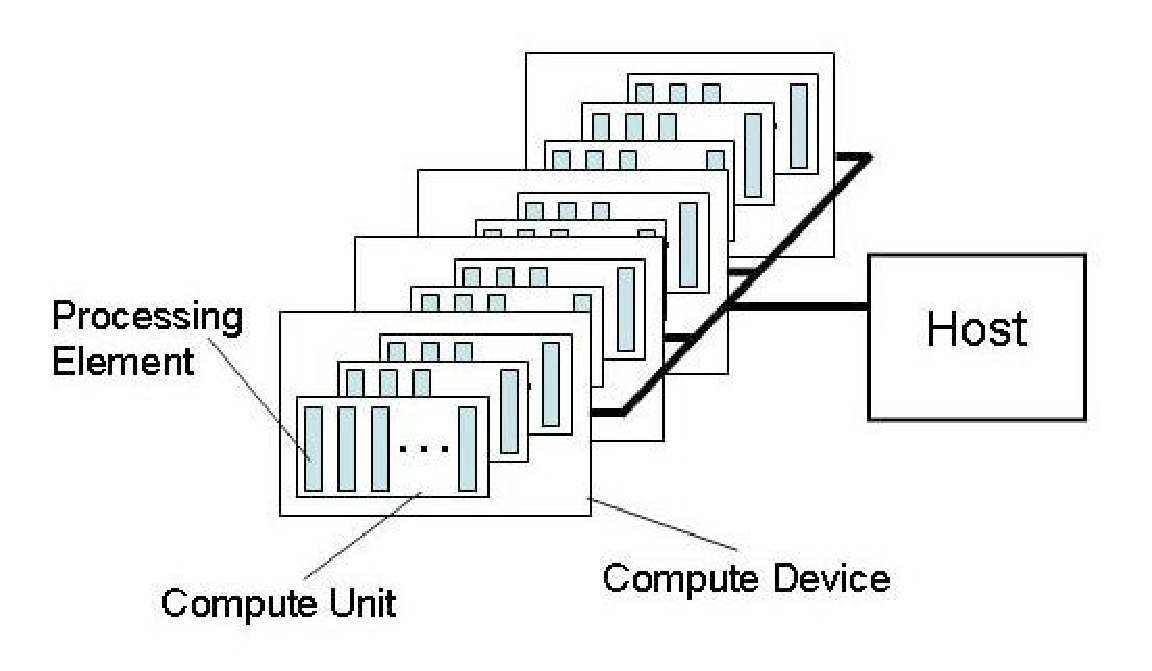
\includegraphics[width=8cm, height=4cm]{./eps/OpenCLArch.eps}
 \caption{OpenCL Architecture}
 \label{fig:OpenCLArch}
\end{figurehere}

\begin{CLCode}
A List containing all the available devices on a system can be obtained calling the \textbf{clGetDeviceIDs()} function. 
\end{CLCode}


\subsubsection{Execution and Index Space}

From a very coarse point of view, we can describe the execution of an OpenCL application as a two-step process:

\begin{enumerate}
	\item the \textbf{host} define the context for \textbf{kernels} and submit them for execution.
	\item the \textbf{kernel} executes on one or more OpenCL device and compute over a stream of data.
\end{enumerate}

In OpenCL, an instance of a kernel is called \textbf{work-item} and it executes over an \textbf{index-space} that is defined every time a new kernel is submitted. We can see the index space as the data domain over which the multiple instances of a kernel may work, and it is also called \textbf{NDRange} (N-dimensional index space, where N is one, two or three). From the graphical point of view of the GPU computation, the index range is no more than the texture on which apply the shader (in fact GPUs normally support 1,2 or 3-dimensional textures).\\

\begin{figurehere}
 \centering
 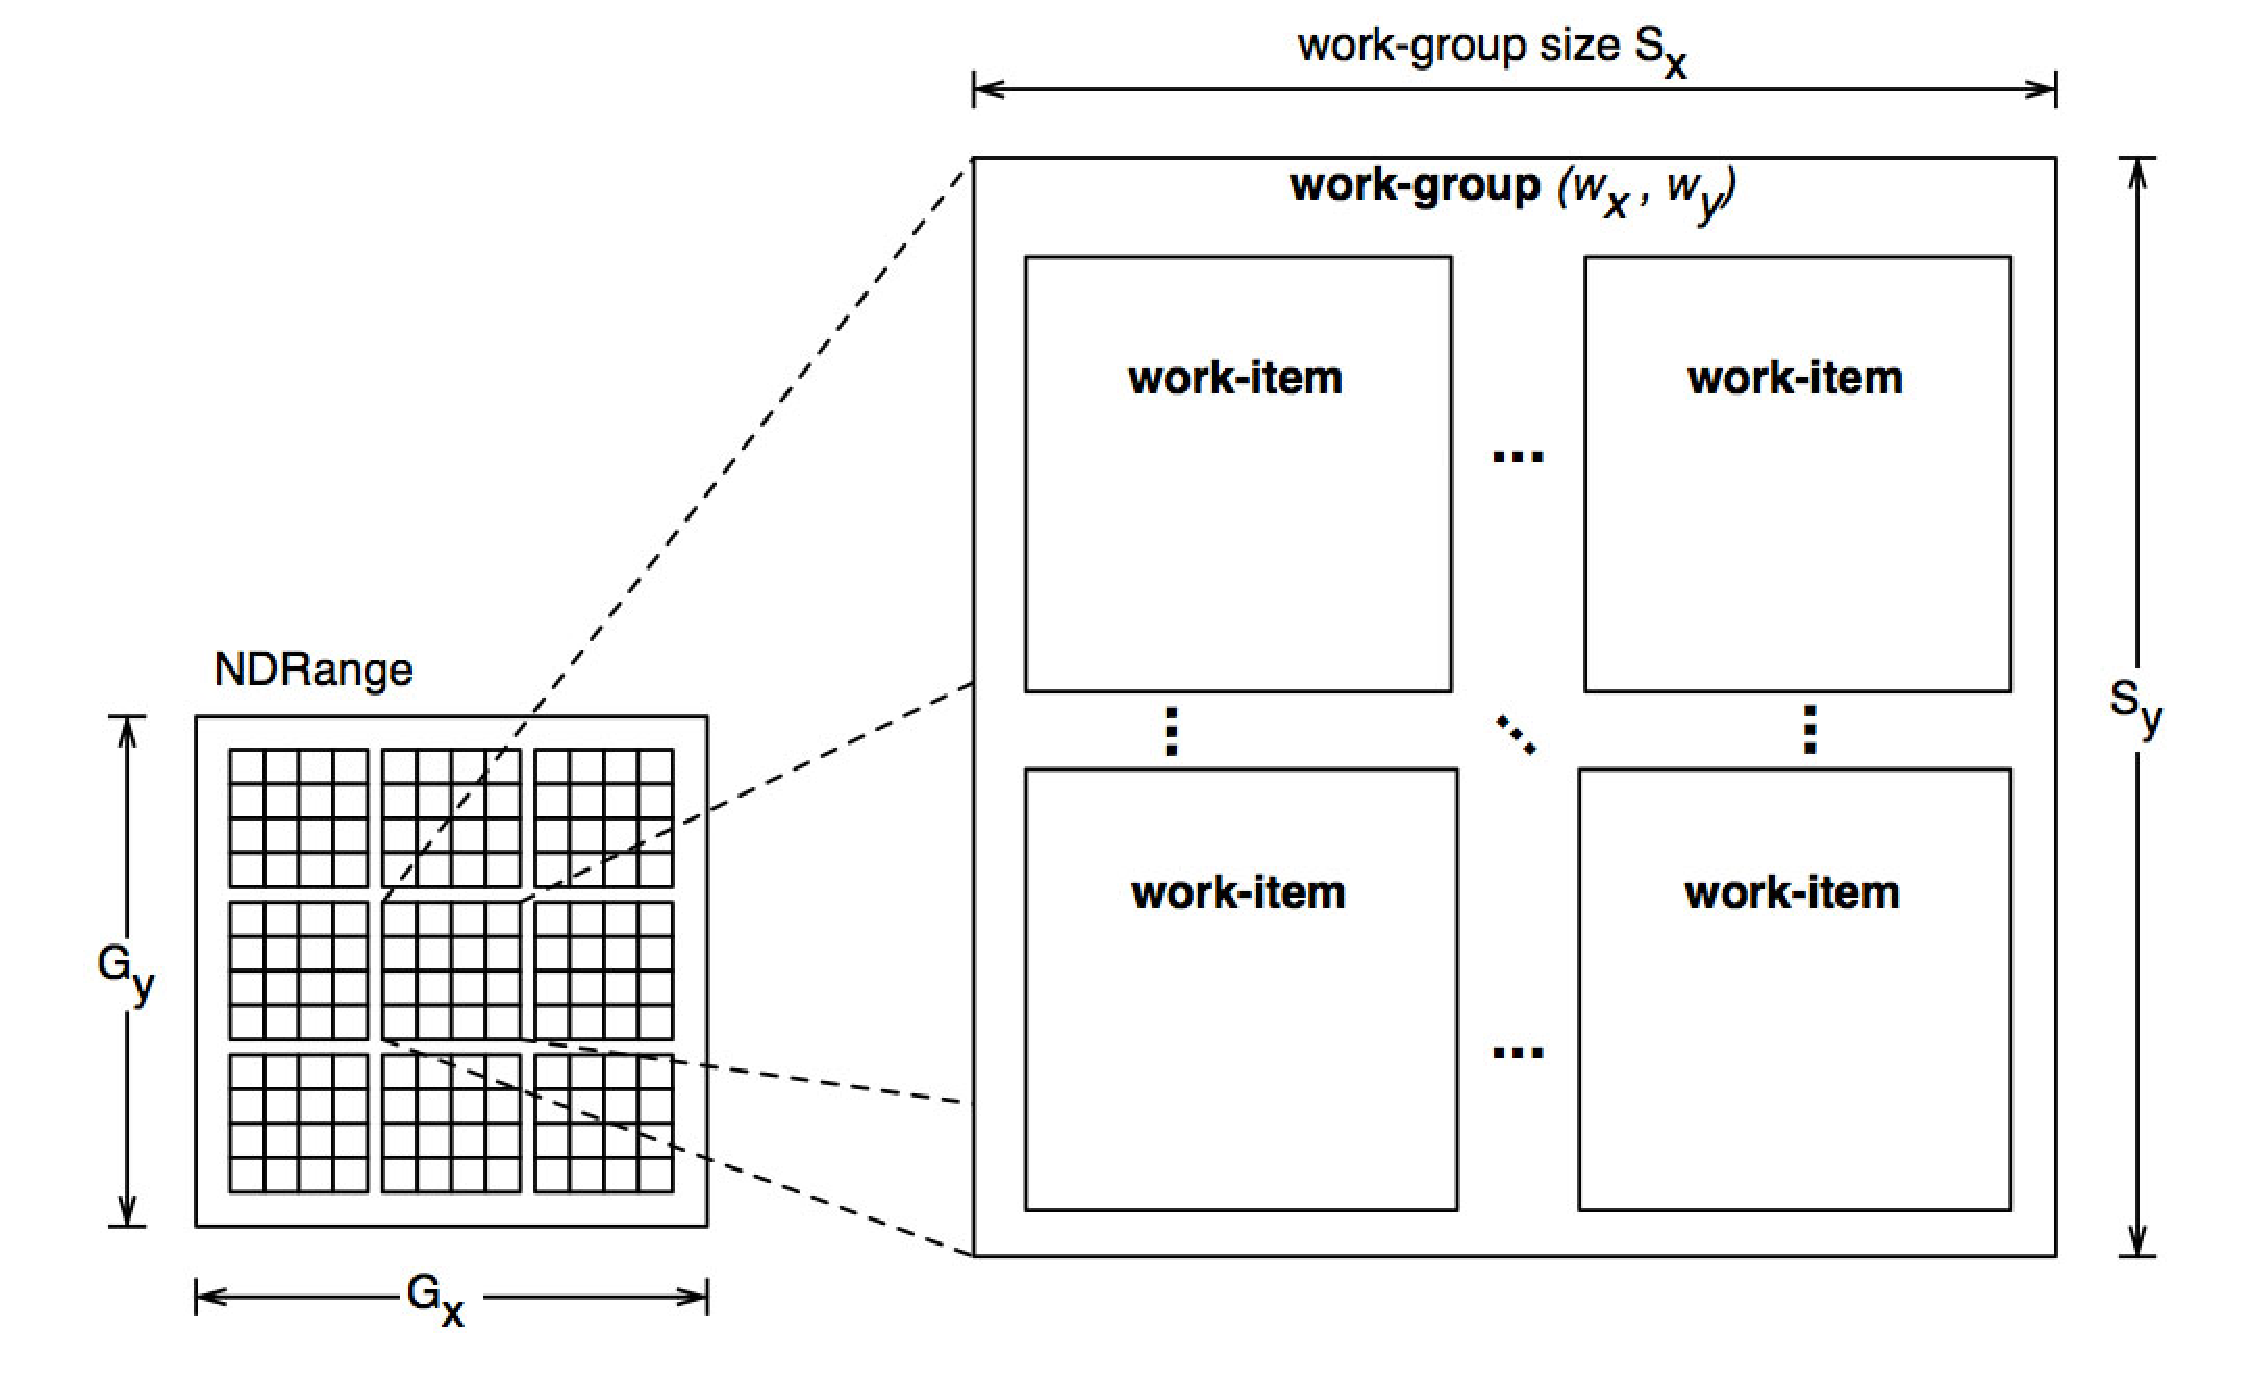
\includegraphics[width=8cm, height=4cm]{./eps/index-space.eps}
 \caption{Work-items mapped over a 2-D NDRange. As you can see, work-items can be organized in Work-Groups. Every work-item has both global and local IDs inside its work-group.}
 \label{fig:indexSpace}
\end{figurehere}

\subsubsection{Kernel Implementation} \label{sect:kernelImplementation}
Mettere esempio implementazione kernel in OpenCL

\subsubsection{Program Context and Command-Queue} \label{sect:context}

When the host defines the \textbf{context} for the application, it basically define four things:

\begin{enumerate}
	\item the collection of OpenCL devices to be used
	\item the collection of functions that will be executed on the devices (that is, the kernels)
	\item \textbf{program objects}, that are simply the source files and executables that implements the kernels
	\item \textbf{memory objects}: the data to be computed
\end{enumerate}

After the context has been created, the host initialize a structure called \textbf{command queue} that is used to schedule commands onto the devices within the context. The command structure is very simple and the main commands issued by the host are only three:

\begin{enumerate}
	\item \textbf{Kernel execution commands}: Execute a kernel on the PEs (Processing Elements) of a device
	\item \textbf{Memory commands}: Transfer data to, from, or between memory objects, or map and unmap
memory objects from the host address space.
	\item	\textbf{Synchronization commands}: Used to specify the order of execution of commands.
\end{enumerate}

\subsubsection{Memory}

There are four types of memory regions in OpenCL: \textbf{Global}, \textbf{Constant}, \textbf{Local} and \textbf{Private}.

\begin{itemize}
	\item Global memory grants read/write access to \textbf{all} the work-items in every work-group.
	\item Constant memory is only used to store constants. Only the host has write privileges over it, while kernels can only read from it.
	\item Local memory is shared among all the work-items that form a group. The host has no access to this memory.
	\item Private memory is allocated directly by the work-item and can be used only by itself. The host has no access to this part of memory.
\end{itemize}

Since computation is carried on parallely, one of the major issues about memory is \textbf{consistency}. OpenCL uses a relaxed consistency memory model: the state of memory visible to a work-item is not guaranteed to be consistent across the collection of work-items at all times. \textbf{Table} \ref{tab:memconsistency} summarizes memory consistency for the various regions of memory available.\\

\begin{tablehere}
{\footnotesize
\begin{tabular}{|p{2cm}|p{5,5cm}|} \hline
\textbf{Memory} & \textbf{Consistency}\\ \hline
Private & memory is not shared, read/write consistency is always guaranteed\\ \hline
Local & consistency is guaranteed between work-items of the same work-group\\ \hline
Global & consistency is guaranteed between work-items of the same work-group, but not between multiple work-groups in the case they are assigned to execute the same kernel\\ \hline
\end{tabular}}
\caption{Memory consistency}
\label{tab:memconsistency}
\end{tablehere}


In OpenCL computation is performed over \textbf{memory objects}. There are two distinct memory objects: \textbf{buffers} and \textbf{images}.

\begin{itemize}
	\item Buffers are used to store a one-dimensional collection of elements (like an array), and those elements can be scalar values (int, float, etc.), vectors or user defined structures.
	Buffers are stored sequentially and \emph{can be accessed using pointers}; elements of a buffer are stored in memory in the \emph{same format} as they are used by kernels (i.e. if the kernel works on single integers, these elements are stored in memory as integers, this is not true for image objects)
	\item Images are used to store bi- or three-dimensional structures and their elements cannot be only selected by a list of predefined image formats (i.e. you cannot simply declare int or floats in an image object). Differently from buffers, elements of images \emph{cannot be accessed directly with a pointer} and they are \emph{always stored in memory as 4-dimensinal vectors} (since graphic shaders work on RGB and Alpha components of the pixels of an image)
\end{itemize}

\begin{CLCode}
In OpenCL memory objects are stored into \textbf{cl\_mem} structs, that can be easily initializated with the \textbf{clCreateBuffer()} and \textbf{clCreateImage()} functions.\\
Image format availables may vary from one graphic adapter to another, a list of supported image formats can be obtained using the \textbf{clGetSupportedImageFormats()} query.
\end{CLCode}





%-----------------------------------------------------------------------------
\subsection{Device Fission Introduction}

Device Fission is an extension of the OpenCL specification (fully defined in the OpenCL 1.2 specification, although is available as an extension of OpenCL 1.1 as well) that allow more control over parallel application.\\
As the term 'fission' implies (the action of dividing or splitting something into two or more parts), device fission allows the sub-dividing of a device into one or more sub-devices. This can be used to control manually which CU (Compute Unit) executes specific openCL commands. This practice, when used carefully, can provide a performance advantage, especially when executing the code on the CPU instead of the GPU.\cite{intel:12:DeviceFission}\\ It is important to note that at present day, \textbf{device fission is not suported on GPUs}.\cite{gaster:11:DeviceFission}
Using device fission does require some knowledge of the underlying target hardware. Device fission should be used carefully and may impact code portability and performance if not used properly.

\subsubsection{Device Fission for Embedded Systems}
Device fissioning can be very useful in an embedded environment (or any other environment where resources are limited) for several reasons:

\begin{itemize}
	\item Device fission allows to use only a \emph{portion} of a device, this means that the OpenCL runtime will not take the entire device for itself and other non-OpenCL application can work on it at the same time.
	\item Device fission can allow specialized memory sharing models (For example see the partitioning by affinity domain described in \textbf{Section} \ref{DF-subdevices})
	\item since embedded systems may have limited graphic capabilities (or no graphic adapter at all), Devide Fission may help to better exploit parallel computation where the only option is to use a CPU and not a GPU
\end{itemize}

\subsubsection{Sub Devices} \label{sect:DF-subdevices}
Each subdevice can have its own \textbf{context} and \textbf{command-queue} (See \textbf{Section} \ref{sect:context})

\begin{CLCode}
In OpenCL you can create new sub-devices using the \textbf{clCreateSubDevices()} function. The first parameter to pass is of type \textbf{cl\_device\_id} and it is the ID of the device that has to be partitioned. You can query for a list of available devices on the system by using the \textbf{clGetDeviceIDs()} function. Each sub-device can have a maximum number of compute units specified by the \textbf{CL\_DEVICE\_PARTITION\_MAX\_COMPUTE\_UNITS} property.
Since sub-devices are treated in the same exact way as "`normal"' devices, different contexts can be created with the \textbf{clCreateContext()} function by simply passing the IDs of the sub-devices.
\label{Code:DevicePartitioning}
\end{CLCode}

There are three main way to partition a device: \textbf{equally}, \textbf{by counts} and \textbf{by affinity domain}.

\begin{itemize}
	\item partitioning a device \textbf{equally} means that the application will try to split the device into as many sub-devices as possible, each containting a number of CUs specified by the programmer. If that number does not divide evenly into the maximum available compute units, the remaining are not used.
	\item \textbf{by counts} means that the device is not divided automatically (and equally), but accordinlgy to a list provided by the programmer (e.g. given the list (4,8,16) the device will be divided into three sub-devices containing respectively 4,8 and 16 CUs)
	\item partitioning by \textbf{affinity domain} is an automatic process that will create sub-devices composed of CUs that share similar levels of cache-hierarchy (specified by the programmer, e.g. L1,L2,L3 caches or NUMA nodes). This can be very useful when micro-management of memory is useful or for system where memory is a critical factor (for example in  embedded systems)
\end{itemize}

You can see examples on how partitioning parameters can be used to create different configurations on the same hardware in \textbf{Appendix A}.\\
Another interesting feature of device fission is that you can partition sub-devices to create a tree-like structure like the one shown in \textbf{Figure \ref{fig:subdevicestree}}:

\begin{figurehere}
 \centering
 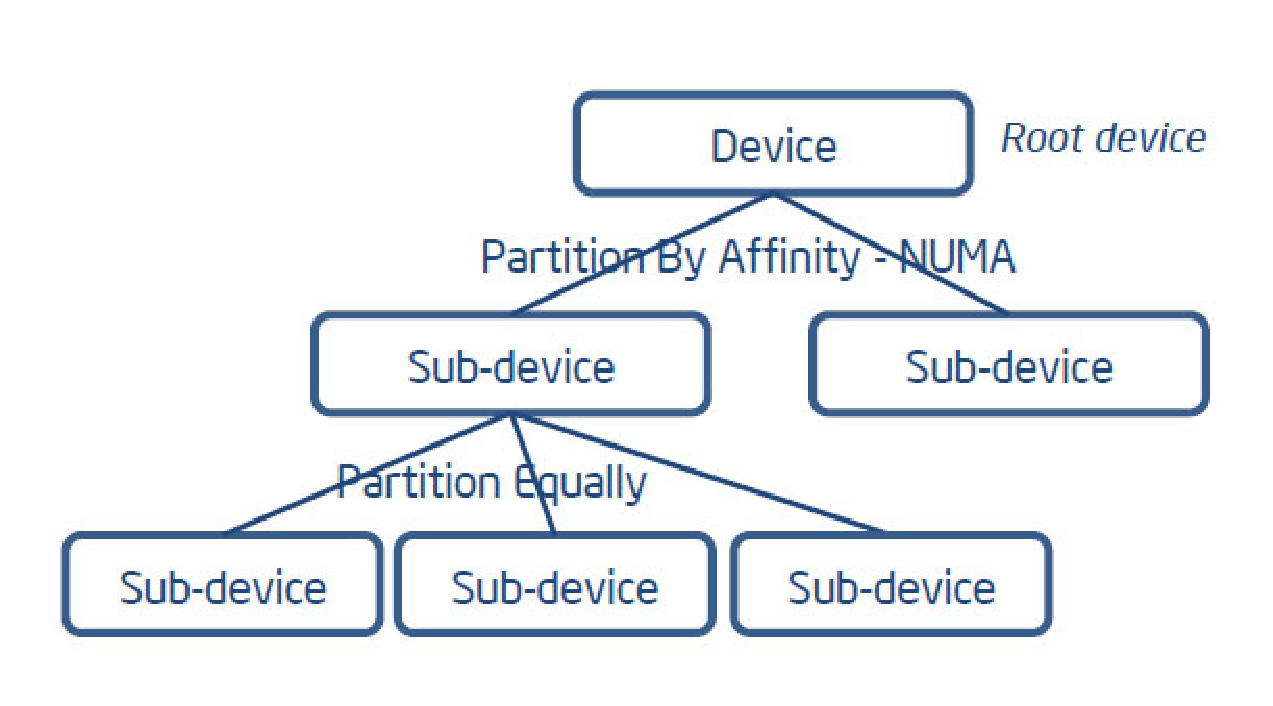
\includegraphics[width=8cm, height=4cm]{./eps/partitionTree.eps}
 \caption{Sub-devices can be further partitioned to create an hierarchy of devices. Each node of the tree can be partitioned using different partition parameters.}
 \label{fig:subdevicestree}
\end{figurehere}

\subsection{Device Fission Strategies}
Device fission can be used in several way to increase performance of OpenCL applications and to manage the (limited) resources of a system in a more efficient way. There are several standard approaches in which device fission can make the difference if used correctly.

\subsubsection{High-Priority dedicated sub-device}
In this scenario, a sub-device is created to deal with critical tasks, while the rest of the device an be used for standard computation.
This configuration can be simply achieved by partitioning the device \textit{by counts}, reserving a few cores for high-priority computation and leaving the rest for normal computation.

{\footnotesize\begin{verbatim}

// Get Device ID from platform [0]
// a list of available platforms can be obtained
// using clGetPlatformIDs() function

clGetDeviceIDs( platforms[0], CL_DEVICE_TYPE_CPU,
                1, &device_id, NULL);
								
// Create two sub-devices, the parameters for the
// partitioning are storend into a 
// cl_device_partition_property array

cl_device_partition_property param[5];
param[0] = CL_DEVICE_PARTITION_BY_COUNTS;
param[1] = 2;   // 1st device: 2 compute units
param[2] = 4; 	// 2nd device: 4 compute units
param[3] = CL_DEVICE_PARTITION_BY_COUNTS_LIST_END;
param[4] = 0; //end of list

//now we can create the sub-devices
cl_device_id output_IDs[2]; 
clCreateSubDevices(device_id, param, 2,
                   output_IDs, NULL);
//our `High Priority' device:
cl_device_id *hpDevice = &output_IDs[0];  
//our `normal' device:    
cl_device_id *normalDevice = &output_IDs[1]; 

\end{verbatim}}

\subsubsection{Memory Proximity}
If the work-items of the application share high amounts of data, it can be useful to create sub-devices that share the same cache or are physically placed on the same NUMA node.
Without device fission, there is no guarantee that the work items will have these characteristics.
This kind of partitioning can be achieved using the \textit{partition by affinity model}, specifying which level of memory needs to be shared.

{\footnotesize\begin{verbatim}
//In this example we will create 8 sub-devices
//that share L3 cache
clGetDeviceIDs( platforms[0], CL_DEVICE_TYPE_CPU,
                1, &device_id, NULL);

// Fill the parameters list
cl_device_partition_property params[3];
params[0] = CL_DEVICE_PARTITION_BT_AFFINITY_DOMAIN;
params[1] = CL_DEVICE_AFFINITY_DOMAIN_L3_CACHE; 
params[2] = 0; // End of list

// Create the sub-devices:
cl_device_id subdevices_IDs[8];
clCreateSubDevices(device_id, params, 8,
                   subdevices_IDs, NULL);
\end{verbatim}}

\subsubsection{Warm Cores Exploitation}
Without device fission, when a new command is submitted to the command-queue it may happen that it is dispatched for execution over a "`cold"' core. A "`cold"' core is one whose caches are filled with data that is not relevant to the current OpenCL program. With device fission we can force to use already "`warmed up"' cores to minimize latency time.
This scenario adapts well for short-running programs, where the overhead of "`warming"' the core is relevant. For long-running programs, using device fission in this way may have very little effect or even degrade performance.
This approach can also be used where thermal management is critical, as it can affect which area of the CPU will heat more.

>>>METTERE ESEMPIO SU COME INDIRIZZARE COMANDI SPECIFICI AL DEVICE

\subsubsection{Maximize Throughput}
This scenario applies when data sharing is very limited or completely absent, and the only important thing is to maintain high levels of throughput. To achieve this, a job must have \textit{all the resources} available for itself (i.e. all the on-chip caches), and no other jobs may interfere, therefore we must create \emph{one and only one} device for each NUMA node, so no device can "`overlap"' resources with another.

SISTEMARE.......Use Partition By Affinity to create N sub-devices one sub-device for each NUMA node.
The sub-devices can then use all NUMA node's resources including all of the available cache.






